\appendix{}

\chapter{Supplemental Material for Chapter \ref{chap:chapter 1}}

All Supplemental Tables can be found in the version 2 bioRxiv preprint at the following location: \href{https://www.biorxiv.org/content/10.1101/2022.06.10.495510v2.supplementary-material}{https://www.biorxiv.org/content/10.1101/2022.06.10.495510v2.supplementary-material}.

\section{Supplementary Figures}
%%%%%%%%%%%%%%%%%%%%%%%%%%%%%%%%%%%%%%%%%%%%%%%%%%%%%%%%%%%%%%%%%%%%%%%%%%%%%%%%

\begin{figure}[h]
    \centering
    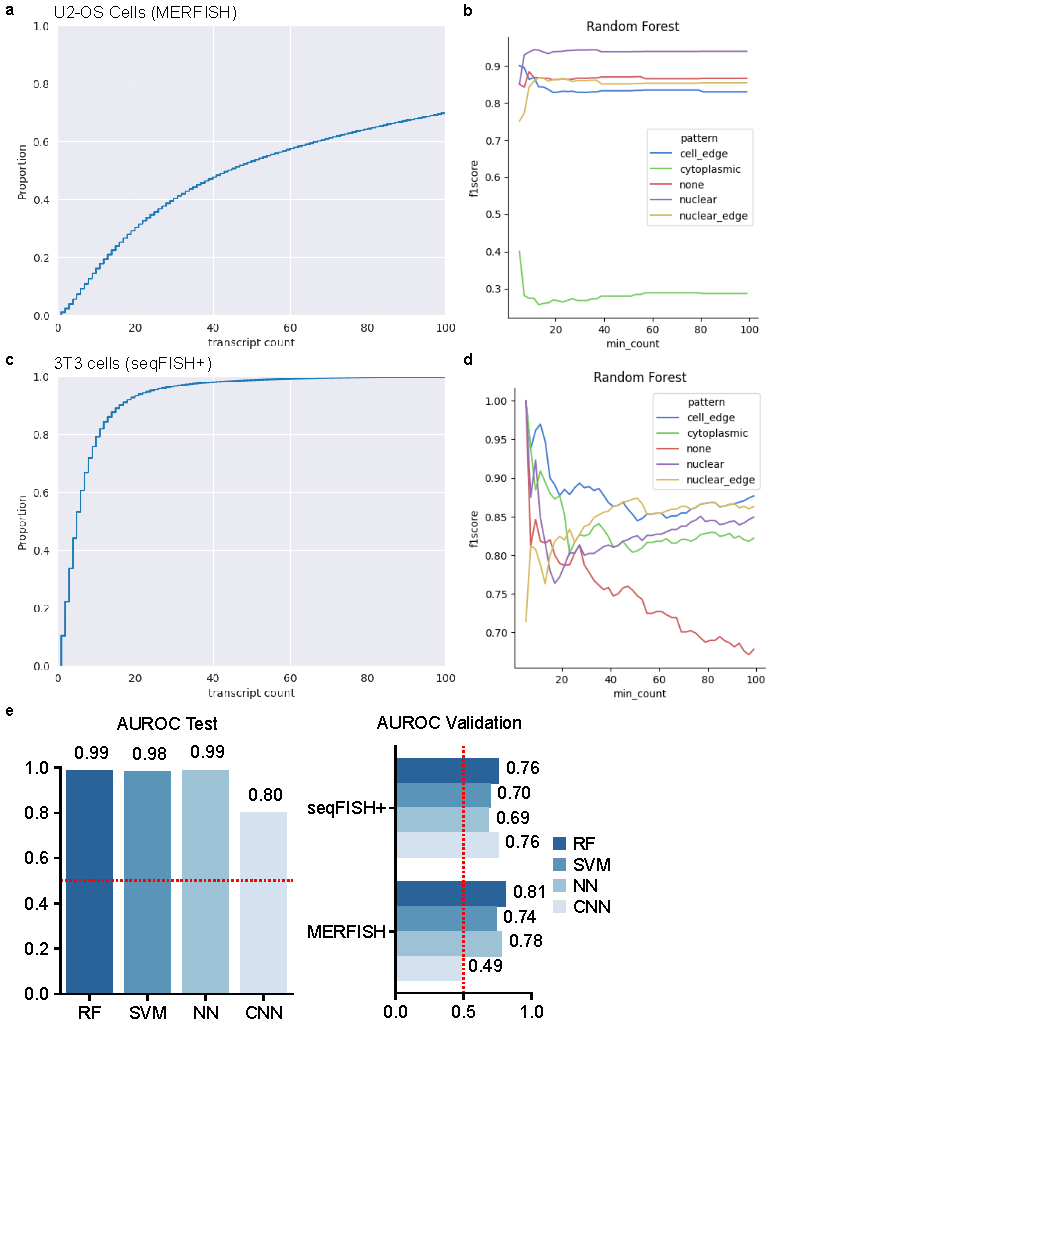
\includegraphics[width=\textwidth]{1_figures-and-files/FigS1.pdf}
    \caption[RNAforest performance evaluation.]{\textbf{RNAforest performance evaluation.} A. Cumulative distribution of sample molecule copy number in U2-OS cells MERFISH dataset. B. Validation F1-score of each binary classifier in RNAforest as a function of sample molecule copy number for MERFISH dataset. C. Cumulative distribution of sample molecule copy number in 3T3 cells seqFISH+ dataset. D. Validation F1-score of each binary classifier in RNAforest as a function of sample molecule copy number for seqFISH+ dataset. E. Benchmarking performance of the 4 base models (RF - random forest, SVM - support vector machine, NN - fully connected neural network, CNN - convolutional neural network), showing AUROC in test and validation data.}\label{fig:supplement rnaforest evaluation}
\end{figure}

\begin{figure}[h]
    \centering
    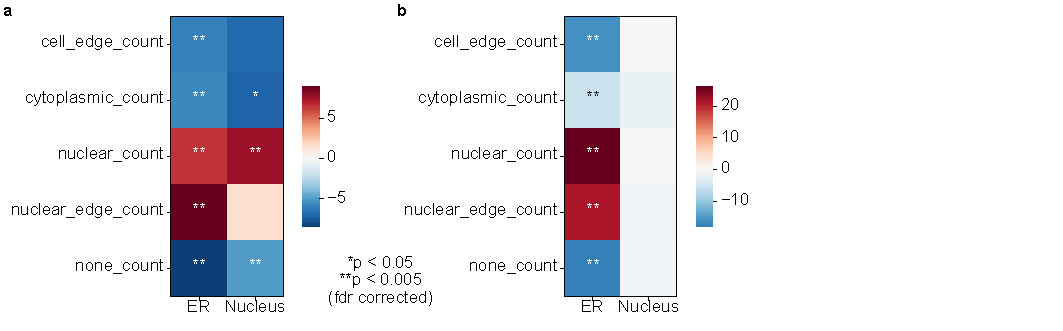
\includegraphics[width=\textwidth]{1_figures-and-files/FigS2.pdf}
    \caption[Enrichment of compartment-specific expression for RNAforest gene pattern frequencies.]{\textbf{Enrichment of compartment-specific expression for RNAforest gene pattern frequencies.} Compartment-specific enrichment of endoplasmic reticulum (ER) and nucleus gene expression – from Xia et al 2019\cite{xiaSpatialTranscriptomeProfiling2019} – relative to RNAforest gene pattern frequencies in the A. MERFISH dataset and B. seqFISH+ dataset. }\label{fig:supplement rnaforest enrichment}
\end{figure}
